% !TEX TS-program = pdflatex
% !TEX encoding = UTF-8 Unicode

% This is a simple template for a LaTeX document using the "article" class.
% See "book", "report", "letter" for other types of document.

\documentclass[11pt]{article} % use larger type; default would be 10pt

\usepackage[utf8]{inputenc} % set input encoding (not needed with XeLaTeX)


%%% PAGE DIMENSIONS
\usepackage{geometry} % to change the page dimensions
\geometry{a4paper} % or letterpaper (US) or a5paper or....


\usepackage{graphicx} % support the \includegraphics command and options

% \usepackage[parfill]{parskip} % Activate to begin paragraphs with an empty line rather than an indent

%%% PACKAGES
\usepackage{booktabs} % for much better looking tables
\usepackage{array} % for better arrays (eg matrices) in maths
\usepackage{paralist} % very flexible & customisable lists (eg. enumerate/itemize, etc.)
\usepackage{verbatim} % adds environment for commenting out blocks of text & for better verbatim
\usepackage{subfig} % make it possible to include more than one captioned figure/table in a single float
\usepackage{cite}
% These packages are all incorporated in the memoir class to one degree or another...

%%% HEADERS & FOOTERS
\usepackage{fancyhdr} % This should be set AFTER setting up the page geometry
\pagestyle{fancy} % options: empty , plain , fancy
\renewcommand{\headrulewidth}{0pt} % customise the layout...
\lhead{}\chead{}\rhead{}
\lfoot{}\cfoot{\thepage}\rfoot{}

%%% SECTION TITLE APPEARANCE
\usepackage{sectsty}
\allsectionsfont{\sffamily\mdseries\upshape} % (See the fntguide.pdf for font help)
% (This matches ConTeXt defaults)

%%% ToC (table of contents) APPEARANCE
\usepackage[nottoc,notlof,notlot]{tocbibind} % Put the bibliography in the ToC
\usepackage[titles,subfigure]{tocloft} % Alter the style of the Table of Contents
\renewcommand{\cftsecfont}{\rmfamily\mdseries\upshape}
\renewcommand{\cftsecpagefont}{\rmfamily\mdseries\upshape} % No bold!

\usepackage{graphicx}
\graphicspath{ {figures} }

\title{Mapping the Brain: An Introduction to Connectomics\\vesiclePy}
\author{Zhou Li, Jizhou Xu, Mary Yen}
%\date{} % Activate to display a given date or no date (if empty),
         % otherwise the current date is printed 

\begin{document}
\maketitle

\section{Abstract}

We have a program capable of mapping the human brain by vesicle clustering available in Matlab. However, this code has many Matlab dependencies and isn't as open-sourced as Python code. Therefore, converting this code into Python code is viable. There are some challenges in that Matlab doesn't translate directly into Python due to differences in data format and dependencies, but we still were able to find a basic pipeline that is able to perform the basic detection actions by using the Python scikit-learn library, RandomForestClassifier to aid in the classifying process of the program. For future work, we would like to do a more complete conversion of vesiclePy. Due to the large size of the program, the complexity of the data, and our team's unfamiliarity with Matlab, doing a basic pipeline was the most realistic goal for a three week course. With more time, we would like to properly learn the algorithms that the Matlab code uses and attempt to improve the code if possible using Python libraries.

\section{Results}

Due to a server problem, the current code takes data from a standalone .mat file, but the Python package does have APIs for downloading data from the ndio server. After splitting the data into a training data set and a testing data set, our programing creates the feature vector by doing calculations with the image data, and then constructs the label vector from the synapses truth data. Because of our unfamiliarity with Matlab, we couldn't perfectly mimic the Matlab implementation on creating the labels, but we have created a skeleton Python file for it for the future. Now, we have all we need for fitting a scikit-learn random forest classifier.\\\\
The mean classification accuracy on the given test data and labels we got was around 99\%. However, since there is only a very small number of synapses in each image, the accuracy here doesn't tell us a lot. We then proceed to calculate the precision and recall of our classifier.\\\\
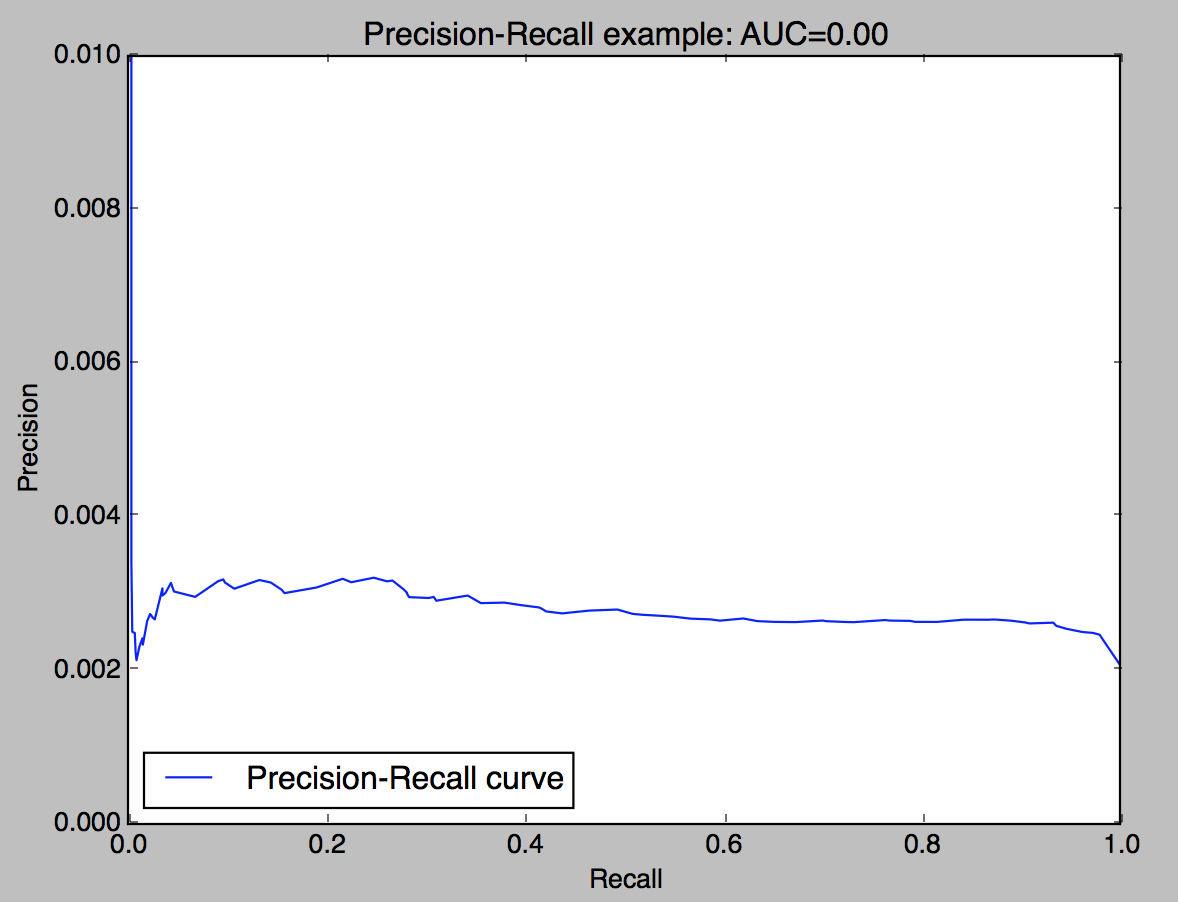
\includegraphics[width=\textwidth]{figures/precision-recall-plot.png}\\\\
We suspect that the reason why the precision is very small is because we only used intensity features for training, and our label generation method is kind of brute-force.

\end{document}

























